\chapter*{Annexes}
\addcontentsline{toc}{chapter}{Annexes}

\section*{Chapitre 2}


\begin{figure}[H]
\centering
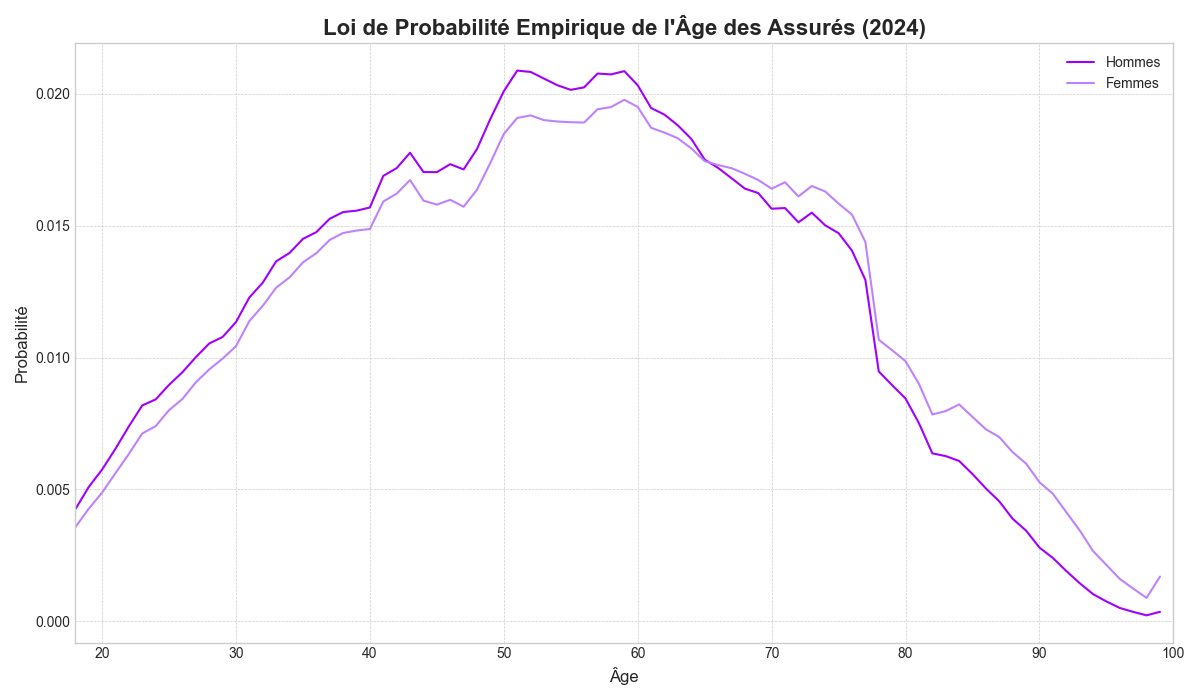
\includegraphics[width=0.9\textwidth]{images/2_chapitres/chapitre3/distribution_age_assures.png}
\caption{Distribution empirique de l'âge des assurés (Hommes et Femmes).}
\label{fig:empirique}
\end{figure}

\begin{figure}[H]
\centering

\includegraphics[width=0.9\textwidth]{images/2_chapitres/chapitre3/estimation_loi_gamma.png}
\caption{Ajustement de la loi Gamma sur la distribution empirique.}
\label{fig:gamma}
\end{figure}

\begin{figure}[H]
\centering
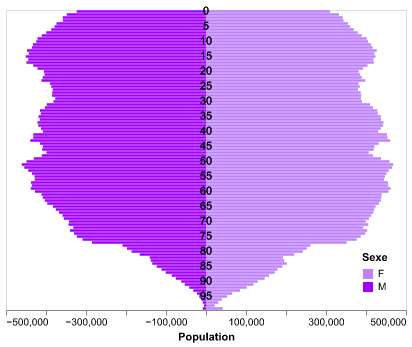
\includegraphics[width=0.9\textwidth]{images/2_chapitres/chapitre3/pyramide_age.png}
\caption{Pyramide des âges de la population française en 2024 \cite{pyramide_age}.}
\label{fig:pyramide_age}
\end{figure}


\begin{table}[H]
  \centering
  \caption{Historique du taux technique maximal et du TMG utilisé dans le modèle (1993--2024)}
  \label{tab:TMG_historique}
  \begin{tabular}{rcc}
    \hline
    Année & $TT^{\max}_t$ & $TMG_t$ \\
          & (taux technique max) & (taux min. garanti retenu) \\
    \hline
    1993 & 0{,}045  & 0{,}045 \\
    1994 & 0{,}045  & 0{,}045 \\
    1995 & 0{,}035  & 0{,}035 \\
    1996 & 0{,}035  & 0{,}035 \\
    1997 & 0{,}0339 & 0{,}0325 \\
    1998 & 0{,}0272 & 0{,}025  \\
    1999 & 0{,}0265 & 0{,}025  \\
    2000 & 0{,}0329 & 0{,}0325 \\
    2001 & 0{,}0301 & 0{,}030  \\
    2002 & 0{,}0292 & 0{,}0275 \\
    2003 & 0{,}0247 & 0{,}0225 \\
    2004 & 0{,}0243 & 0{,}0225 \\
    2005 & 0{,}0207 & 0{,}020  \\
    2006 & 0{,}0229 & 0{,}0225 \\
    2007 & 0{,}0260 & 0{,}025  \\
    2008 & 0{,}0261 & 0{,}025  \\
    2009 & 0{,}0219 & 0{,}020  \\
    2010 & 0{,}0189 & 0{,}0175 \\
    2011 & 0{,}0213 & 0{,}020  \\
    2012 & 0{,}0153 & 0{,}015  \\
    2013 & 0{,}0141 & 0{,}0125 \\
    2014 & 0{,}0099 & 0{,}0075 \\
    2015 & 0{,}0051 & 0{,}0000 \\
    2016 & 0{,}0027 & 0{,}0000 \\
    2017 & 0{,}0045 & 0{,}0000 \\
    2018 & 0{,}0048 & 0{,}0000 \\
    2019 & 0{,}0009 & 0{,}0000 \\
    2020 & 0{,}0000 & 0{,}0000 \\
    2021 & 0{,}0003 & 0{,}0000 \\
    2022 & 0{,}0090 & 0{,}0000 \\
    2023 & 0{,}0186 & 0{,}0000 \\
    2024 & 0{,}0180 & 0{,}0000 \\
    \hline
  \end{tabular}
\end{table}

\subsection*{Calibration initiale du modèle d'allocation (Inclusion de l'ancienneté)}
\phantomsection\label{annexe:anciennete}

Lors de la phase de spécification du modèle Logit visant à répartir la Provision Mathématique entre le fonds en euros et les unités de compte, une troisième variable explicative avait été initialement retenue : l'ancienneté du contrat ($\text{Anciennete}_i$). L'objectif était de capter un effet générationnel, l'hypothèse économique sous-jacente étant que les contrats les plus anciens (souscrits dans un contexte de taux garantis élevés) étaient structurellement plus orientés vers le fonds en euros. Le prédicteur linéaire s'écrivait alors :
\begin{equation*}
    \eta_i = \beta_0 + \beta_{\text{age}} \, \text{Age}_i + \beta_{\text{pm}} \, \log(\text{PM}_i) + \beta_{\text{anc}} \, \text{Anciennete}_i
\end{equation*}

Cependant, la calibration par \textit{matching de moments} sur les profils de contrôle a abouti aux coefficients suivants : $\beta_0 = 1.0039$, $\beta_{\text{age}} = -0.0424$, $\beta_{\text{pm}} = 0.0746$ et $\beta_{\text{anc}} = 0.0008$.

Outre sa valeur quasi nulle traduisant un pouvoir explicatif marginal, le signe positif du coefficient $\beta_{\text{anc}}$ contredisait l'intuition économique de départ. Ce résultat s'explique par une forte colinéarité entre l'âge de l'assuré et l'ancienneté de son contrat. L'algorithme d'optimisation a par conséquent transféré l'essentiel du poids explicatif sur la variable d'âge, rendant l'ancienneté redondante. Par souci de robustesse et pour éviter tout sur-paramétrage (\textit{overfitting}), cette variable a donc été retirée du modèle final présenté dans le corps du mémoire.